\documentclass[conference]{IEEEtran}

% Paquetes esenciales
\usepackage[utf8]{inputenc}
\usepackage[T1]{fontenc}
\usepackage[spanish]{babel}
\usepackage{geometry}
\usepackage{graphicx}
\usepackage{float}
\usepackage{booktabs}
\usepackage{longtable}
\usepackage{array}
\usepackage{amsmath}
\usepackage{amssymb}
\usepackage{xcolor}
\usepackage{caption}
\usepackage{subcaption}
\usepackage{fancyhdr}
\usepackage{titlesec}
\usepackage{parskip}
\usepackage{enumitem}
\usepackage{multirow}
\usepackage{tabularx}
\usepackage{microtype}
\usepackage[backend=bibtex, authoryear]{natbib}  % Para citas autor-año

% Configuración de geometría para dos columnas
\geometry{top=2.5cm, bottom=2.5cm, left=2.2cm, right=2.2cm, columnsep=0.8cm}

% Encabezado simple para estilo de paper
\pagestyle{plain}

% Título y autores
\title{
  \textbf{Análisis visual del rendimiento de futbolistas mediante un sistema de puntuación objetiva y \textit{embedding} profundo con agrupamiento difuso}\\
}
\author{
    Sergio Sebastian Santos Mena Quispe
}
\date{Junio 2026}

\begin{document}

  \maketitle
  \begin{abstract}
    La evaluación del rendimiento de los jugadores de fútbol se ha sustentado tradicionalmente en metodologías observacionales y calificaciones subjetivas emitidas por expertos, introduciendo sesgos cognitivos y alta varianza en el análisis. Siguiendo la taxonomía de tareas analíticas propuesta por \citeauthor{evers2024visual} (\citeyear{evers2024visual}), este artículo presenta \textit{StatsBomb Scout Analytics}, un sistema de análisis visual interactivo que computa métricas de rendimiento objetivas basadas en datos espacio-temporales y de eventos para pases, duelos y tiros. La infraestructura tecnológica integra repositorios de datos abiertos, un \textit{pipeline} de procesamiento analítico en línea (OLAP) optimizado para latencia sub-segundo, y una arquitectura orientada a servicios. Como extensión metodológica original, se propone un \textit{embedding} profundo del rendimiento bajo el marco de \textit{Deep Embedded Clustering} (DEC) propuesto por \citeauthor{demir2026how} (\citeyear{demir2026how}), que combina un autocodificador simétrico con un refinamiento por divergencia KL para producir un espacio latente de diez dimensiones donde se asienta un agrupamiento difuso. La selección final del método de agrupamiento sobre ese espacio latente se respalda en el marco de validación compuesta de \citeauthor{akhanli2022clustering} (\citeyear{akhanli2022clustering}), que benchmarkéa cinco métodos clásicos contra \textit{clusterings} aleatorios calibrados y produce un índice agregado $A_1$. El clustering híbrido adoptado genera perfiles tácticos latentes con pertenencias difusas, diseñados para optimizar tareas de \textit{scouting} comparativo y detección de roles híbridos. La validación empírica del sistema se demuestra mediante cinco casos de estudio sobre datos abiertos de \textit{StatsBomb}, corroborando y extendiendo hallazgos previos en la literatura de la analítica deportiva.
  \end{abstract}
  \vspace{1em}
\begin{IEEEkeywords}
análisis visual de datos, analítica deportiva, modelado de rendimiento, métricas objetivas, \textit{Deep Embedded Clustering}, agrupamiento difuso, fútbol.
\end{IEEEkeywords}
  \vspace{2em}

%% ============================================================================
\section{Introducción}
% ============================================================================

El fútbol profesional contemporáneo está experimentando una revolución digital sin precedentes, impulsada por la adopción masiva de tecnologías de posicionamiento y el registro minucioso de eventos tácticos. En la actualidad, cada encuentro genera millones de coordenadas espaciotemporales y miles de registros estructurados que capturan con precisión quirúrgica las interacciones dinámicas entre los veintidós jugadores y el balón \citep{janetzko2014feature, anzer2021goal}. Este ecosistema de datos masivos (*big data*) ha transformado radicalmente la gestión deportiva en los clubes de élite. Los departamentos de ciencias del deporte, los directores técnicos y las secretarías técnicas ya no dependen únicamente de la intuición o de la observación pasiva, sino que demandan el modelado matemático de los patrones de juego y del comportamiento espacial para extraer ventajas competitivas sostenibles dentro y fuera del terreno de juego \citep{zhao2017visual, stein2019where}.

La motivación detrás de esta investigación converge en dos frentes críticos: el institucional-deportivo (impacto social y de negocio) y el tecnológico (computacional). Desde la perspectiva del *scouting* y la dirección técnica, el impacto económico y deportivo de una contratación errónea o de un planteamiento táctico deficiente es crítico; optimizar el proceso de selección mediante la identificación de perfiles que encajen con precisión en sistemas tácticos específicos representa una necesidad imperativa para mitigar riesgos financieros y potenciar el rendimiento colectivo del club. Desde el punto de vista computacional, el desafío radica en el hecho de que estos grandes volúmenes de datos crudos y heterogéneos suelen quedar subutilizados debido a su baja abstracción y alta complejidad algorítmica. Transformar estos flujos masivos en interfaces visuales analíticas reactivas e interactivas en tiempo real representa un avance tecnológico sustancial. Esto permite democratizar el uso de modelos estadísticos complejos, facilitando que los tomadores de decisiones en el área deportiva exploren métricas avanzadas sin requerir conocimientos profundos en programación \citep{perin2013soccerstories, evers2024visual}.

A pesar de esta abundancia de datos, la evaluación del rendimiento de los futbolistas en los procesos de dirección técnica y reclutamiento continúa dependiendo en gran medida de observaciones subjetivas y calificaciones emitidas por analistas o expertos. Esta dependencia introduce sesgos cognitivos, variabilidad entre evaluadores y serias dificultades para realizar comparaciones consistentes entre jugadores que operan en diferentes ligas o contextos tácticos \citep{hvattum2019comprehensive, evers2024visual}. Paralelamente, el fútbol moderno genera volúmenes masivos de datos espacio-temporales y de eventos que, pese a su potencial para proporcionar evaluaciones objetivas, aún no son aprovechados de manera integral en herramientas que faciliten el análisis del rendimiento individual de cara al usuario final. Asimismo, los procesos de *scouting* y búsqueda de talentos suelen requerir la comparación de jugadores con características tácticas similares, una tarea que resulta exponencialmente compleja cuando se dispone de una gran cantidad de información y no existen mecanismos computacionales que permitan identificar automáticamente perfiles de juego comparables. En consecuencia, persiste la necesidad de contar con una plataforma basada en datos que integre métricas objetivas de rendimiento, técnicas de visualización analítica y métodos de agrupamiento de jugadores para apoyar la toma de decisiones en el análisis estratégico y el *scouting* deportivo.

Para resolver esta problemática, el objetivo principal de este trabajo es desarrollar y formalizar \textit{StatsBomb Scout Analytics}, una plataforma visual-analítica diseñada para facilitar la evaluación, comparación y *scouting* de futbolistas mediante la integración de métricas objetivas de rendimiento, interfaces interactivas y técnicas de agrupamiento multivariante (*clustering*) basadas en datos espacio-temporales y eventos de juego. Al operacionalizar y extender el marco de trabajo de tareas analíticas propuesto por \citeauthor{evers2024visual} (\citeyear{evers2024visual}), este sistema busca proveer a los directores técnicos y cazatalentos de un instrumento computacional riguroso que minimice la subjetividad inherente al análisis tradicional, contribuyendo a una toma de decisiones más consistente, transparente y estrictamente guiada por datos (*data-driven*) en el ámbito del fútbol profesional.


% ============================================================================
\section{Trabajos Relacionados}
% ============================================================================

El análisis de datos en el fútbol profesional se ha abordado desde múltiples disciplinas. Desde la perspectiva metodológica, la literatura previa puede clasificarse en dos grandes enfoques: métodos basados en modelado matemático y extracción de características (Machine Learning), y métodos enfocados en la visualización analítica. 

\subsection{Modelado de Rendimiento y Machine Learning}
La extracción de características y la predicción de rendimiento han evolucionado desde métricas estadísticas básicas hacia modelos algorítmicos complejos. \citeauthor{hvattum2019comprehensive} (\citeyear{hvattum2019comprehensive}) proporciona una revisión exhaustiva de los modelos de regresión y regularización matemática para las métricas de \textit{plus-minus}, diseñadas para distribuir el crédito del equipo a los jugadores individuales de forma objetiva. Para estimar el valor de los eventos en un espacio continuo, \citeauthor{zhao2017visual} (\citeyear{zhao2017visual}) proponen modelar los partidos como un Proceso de Recompensa de Markov (MRP) resolviéndolo mediante \textit{Random Forests}, lo que permite extraer periodos de alta intensidad de juego. Por su parte, \citeauthor{anzer2021goal} (\citeyear{anzer2021goal}) demuestran que la integración de datos posicionales y de eventos en un modelo \textit{Extreme Gradient Boosting} (XGBoost) mejora drásticamente la predicción de la probabilidad de gol (xG) superando a las métricas tradicionales. Asimismo, para la abstracción de comportamientos, \citeauthor{janetzko2014feature} (\citeyear{janetzko2014feature}) aplican algoritmos de agrupamiento como K-Means y DBSCAN para segmentar fases de actividad individual a partir de vectores numéricos. De manera más reciente y estrechamente alineada con nuestra investigación, \citeauthor{pacifico2025fuzzy} (\citeyear{pacifico2025fuzzy}) propone un marco analítico que utiliza agrupamiento difuso (\textit{fuzzy clustering}) junto con modelos de aprendizaje interpretable para extraer perfiles latentes de rendimiento ofensivo y evaluar la resiliencia y versatilidad de los jugadores en diferentes competiciones.

Más cercano todavía a la propuesta de este trabajo, \citeauthor{demir2026how} (\citeyear{demir2026how}) introduce un \textit{pipeline} basado en \textit{Deep Embedded Clustering} (DEC) para descubrir estilos de juego a partir de datos de eventos: un autocodificador simétrico se pre-entrena con error cuadrático medio y se refina posteriormente mediante una pérdida de divergencia KL entre una asignación suave $q_{ij}$ (núcleo t de Student) y un objetivo $p_{ij}$ de mayor nitidez, aprendiendo conjuntamente representación y agrupamiento. Demir et al. segmentan los partidos en cuatro fases posesionales (In-Possession, Out-of-Possession, Positive Transition, Negative Transition) y construyen 30 características atacantes y 45 defensivas por equipo-partido-fase. Su \textit{framework} produce, sin embargo, etiquetas \textit{crisp} (asignación argmax) por equipo-partido, agregadas por \textit{votación mayoritaria} al equipo. Por su parte, \citeauthor{akhanli2022clustering} (\citeyear{akhanli2022clustering}) abordan la selección del método de agrupamiento en datos de futbolistas mediante un índice compuesto y calibrado, $A(\mathcal{C})$, agregación de cinco criterios (disimilitud intra-clúster media, índice de separación, $\Gamma$ de Pearson, entropía de Shannon y \textit{Bootstab}) sobre \textit{clusterings} aleatorios como referencia nula. Su enfoque es el que adoptamos como respaldo estadístico para seleccionar entre métodos clásicos aplicados al espacio latente DEC, en lugar de aceptar a priori una configuración fija como k=4 o k=8.

\textbf{Limitaciones:} Aunque la eficacia y precisión predictiva de estos métodos ha sido comprobada, la mayoría se enfoca exclusivamente en tareas de análisis estático u \textit{offline} y carecen de un proceso de análisis visual interactivo \citep{hvattum2019comprehensive, anzer2021goal, pacifico2025fuzzy}. Esto dificulta que expertos del dominio (como los \textit{scouts}) puedan explorar dinámicamente la evolución táctica, ajustar parámetros en tiempo real o integrar su conocimiento de forma visual.

\subsection{Visualización Analítica en el Fútbol}
Para acercar los datos complejos a los usuarios finales, la analítica visual ha cobrado gran relevancia. \citeauthor{perin2013soccerstories} (\citeyear{perin2013soccerstories}) introdujeron \textit{SoccerStories}, un sistema que agrupa fases del partido en narrativas visuales interactivas orientadas a facilitar la comunicación táctica. \citeauthor{benitosantos2018data} (\citeyear{benitosantos2018data}) desarrollaron un prototipo exploratorio que permite el análisis del comportamiento táctico colectivo, evaluando métricas como la dispersión y los centroides del equipo sobre el terreno de juego. Profundizando en la interactividad, \citeauthor{stein2019where} (\citeyear{stein2019where}) incorporaron análisis contrafácticos ("\textit{what-if}"), permitiendo a los analistas reposicionar jugadores manualmente para evaluar cómo cambiarían los espacios libres y las opciones de pase. De manera fundamental para nuestra investigación, \citeauthor{evers2024visual} (\citeyear{evers2024visual}) propusieron una herramienta de analítica visual basada en calificaciones objetivas de rendimiento (pases, duelos y tiros), en la cual los usuarios pueden ajustar interactivamente los pesos de cada métrica mediante gráficos de radar para adaptarse a diferentes perfiles posicionales.

\textbf{Limitaciones:} Sin embargo, gran parte de estos enfoques visuales se centran en el análisis de micro-eventos o en la evaluación de fases de un único partido, sin abstraer a los jugadores en perfiles macroscópicos \citep{perin2013soccerstories, stein2019where, benitosantos2018data}. Si bien el marco de \citeauthor{evers2024visual} (\citeyear{evers2024visual}) es sumamente flexible para la evaluación individual, carece de una capa de aprendizaje no supervisado que asista en la búsqueda y agrupamiento automático de perfiles similares, lo cual es una necesidad imperativa en los departamentos de \textit{scouting}.

\subsection{Contextualización de Nuestra Propuesta}
A diferencia de los trabajos anteriores, nuestra propuesta, \textit{StatsBomb Scout Analytics}, se sitúa en la intersección ideal de tres líneas: la calificación objetiva de \citeauthor{evers2024visual} (\citeyear{evers2024visual}), el \textit{embedding} profundo con refinamiento KL de \citeauthor{demir2026how} (\citeyear{demir2026how}), y la validación compuesta de \citeauthor{akhanli2022clustering} (\citeyear{akhanli2022clustering}). Tomando como base la estructura de evaluación objetiva y las interfaces analíticas interactivas de \citeauthor{evers2024visual}, integramos el \textit{embedding} DEC como espacio de representación y el marco $A_1$ de \citeauthor{akhanli2022clustering} como criterio cuantitativo para seleccionar el agrupamiento sobre ese espacio. Sobre la representación DEC aplicamos un algoritmo de agrupamiento difuso (\textit{Fuzzy C-Means}) para producir vectores de pertenencia suave por jugador, inspirándonos en la capacidad de perfilado latente demostrada por \citeauthor{pacifico2025fuzzy} (\citeyear{pacifico2025fuzzy}). Esta combinación aborda directamente las brechas identificadas en la literatura: los perfiles no se etiquetan de forma rígida sino con membresías continuas, la selección del método y del número de clústeres no es arbitraria sino empíricamente calibrada, y el sistema no solo provee visualizaciones multi-nivel para evaluar a un jugador, sino que automatiza la inferencia de sub-perfiles tácticos (con $k=8$), facilitando las búsquedas comparativas complejas que exige el \textit{scouting} moderno.

\subsection{Cuadro Resumen Comparativo}

A continuación, la Tabla \ref{tab:related_works} resume y contrasta las características metodológicas de la literatura analizada, posicionando el aporte de nuestro sistema.

\begin{table*}
\centering
\caption{Resumen comparativo de trabajos relacionados frente a nuestra propuesta}
\label{tab:related_works}
\footnotesize
\setlength{\tabcolsep}{4pt}
\begin{tabular}{@{}p{2.3cm} p{2.2cm} p{1.8cm} p{2.5cm} p{1.4cm} p{2.7cm}@{}}
\toprule
\textbf{Investigación} & \textbf{Enfoque Principal} & \textbf{Tipo de Datos} & \textbf{Uso de ML / Clustering} & \textbf{Interactividad Visual} & \textbf{Vacío / Limitación Abordada} \\ \midrule
\citeauthor{janetzko2014feature} (\citeyear{janetzko2014feature}) & Extracción Características & Posicionales & Sí (K-Means, DBSCAN) & Media & Falta métricas de rendimiento globales. \\
\citeauthor{zhao2017visual} (\citeyear{zhao2017visual}) & Modelado Estadístico (MRP) & Espaciotemporales & Sí (Random Forest) & Baja & Solo evaluación matemática, no scouting. \\
\citeauthor{anzer2021goal} (\citeyear{anzer2021goal}) & Predicción de xG & Posicionales y Eventos & Sí (XGBoost) & Baja & Modelo cerrado, sin perfiles tácticos. \\
\citeauthor{stein2019where} (\citeyear{stein2019where}) & Visualización Contrafáctica & Trayectorias & No & Alta & Micro-táctica, no evaluación de talento. \\
\citeauthor{pacifico2025fuzzy} (\citeyear{pacifico2025fuzzy}) & Perfilado y Resiliencia & Índices Compuestos & Sí (Fuzzy Clustering, XGBoost) & Baja & Carece de un tablero interactivo de exploración visual. \\
\citeauthor{demir2026how} (\citeyear{demir2026how}) & DEC + estilos de juego & Eventos & Sí (AE + KL-refinement) & Nula & Etiquetas \textit{crisp}; enfocado en equipo, no en jugador. \\
\citeauthor{akhanli2022clustering} (\citeyear{akhanli2022clustering}) & Validación de clustering & Variables mixtas & Sí (PAM, Ward, Spectral) & Nula & Sólo selección de método; sin visualización. \\
\citeauthor{evers2024visual} (\citeyear{evers2024visual}) & Calificaciones Objetivas & Eventos & No (Regresión logística) & Alta & \textbf{Carece de clustering para comparar perfiles latentes.} \\ \midrule
\textbf{Nuestra Propuesta} & \textbf{Visual Analytics + Scouting} & \textbf{Eventos (StatsBomb)} & \textbf{Sí (DEC + FCM)} & \textbf{Alta} & \textbf{Integra calificaciones interactivas con \textit{embedding} DEC y clustering difuso $k=8$ respaldado por el índice $A_1$.} \\ \bottomrule
\end{tabular}
\end{table*}


% ============================================================================
\section{Modelos Metodológicos y Algorítmicos}
% ============================================================================

El objetivo central de esta investigación es transicionar desde un análisis subjetivo hacia una evaluación computacional robusta. Para lograrlo, el sistema propuesto se fundamenta en la integración de tres pilares metodológicos: (i) la calificación objetiva evento por evento de \cite{evers2024visual}; (ii) el \textit{embedding} profundo mediante \textit{Deep Embedded Clustering} (DEC) de \cite{demir2026how}, que aprende un espacio latente de diez dimensiones a partir de un autocodificador refinado con divergencia KL; y (iii) el agrupamiento difuso \textit{Fuzzy C-Means} (FCM) \cite{pacifico2025fuzzy} sobre ese espacio latente, cuya configuración se respalda en el índice compuesto $A_1$ de \cite{akhanli2022clustering}. A continuación, se detallan los fundamentos teóricos, la arquitectura matemática de cada componente y la diferenciación de nuestra propuesta.

\subsection{Bases Teóricas y Conceptos Clave}
El análisis de rendimiento en el fútbol requiere la abstracción de eventos discretos (un pase, un tiro, un duelo) en vectores de características numéricas. Clásicamente, la agrupación de jugadores para tareas de \textit{scouting} se ha realizado mediante algoritmos de partición dura o estricta (\textit{hard clustering}), como K-Means \cite{janetzko2014feature}. En estos modelos, un jugador es asignado a un único clúster táctico (por ejemplo, "Defensa Central"). Sin embargo, el fútbol moderno se caracteriza por la versatilidad; un lateral puede tener funciones de extremo o un mediocampista puede actuar como falso nueve. Para capturar esta complejidad, introducimos la teoría de los conjuntos difusos (\textit{Fuzzy Sets}), la cual permite que un elemento pertenezca a múltiples conjuntos simultáneamente con diferentes grados de membresía.

\subsection{Formulación de las Calificaciones Objetivas de Rendimiento}
\label{subsec:calificaciones}

Antes de describir el algoritmo de agrupamiento, es necesario precisar el origen del vector de características $x_i \in \mathbb{R}^d$ que alimenta al modelo FCM, puesto que la calidad del agrupamiento depende directamente de la calidad de las calificaciones individuales que lo componen. Estas calificaciones se adoptan directamente del marco propuesto por \citeauthor{evers2024visual} (\citeyear{evers2024visual}), quienes definen un esquema de puntuación granular evento por evento que, en una etapa posterior, se agrega estadísticamente por jugador y por partido. A continuación se detalla la formulación matemática completa, dado que constituye el cimiento sobre el cual se construyen tanto la capa interactiva de ponderación (T2) como la capa de agrupamiento difuso (T4) de nuestra propuesta.

\textbf{Esquema general de agregación.} Cada evento individual (un pase, un duelo o un tiro) recibe, en primer lugar, una o varias calificaciones $r_{k,i} \in [0,10]$, donde $k \in \{p,d,s\}$ identifica el tipo de evento (pases, duelos o tiros, respectivamente) e $i$ indexa la sub-métrica considerada. Estas calificaciones elementales se combinan en un promedio ponderado por jugador y partido, de modo que el puntaje agregado para cada categoría se obtiene como

\begin{equation}
S_k = \frac{\sum_{i=1}^{N_k} w_{k,i}\, r_{k,i}}{\sum_{i=1}^{N_k} w_{k,i}},
\label{eq:Sk}
\end{equation}

donde $N_k$ es el número de calificaciones disponibles para el tipo de evento $k$ y $w_{k,i}$ es el peso definido por el usuario para la sub-métrica $i$ (Vista 1, T2). Finalmente, el puntaje global del jugador surge de combinar las tres categorías mediante un segundo promedio ponderado:

\begin{equation}
S = \frac{w_p S_p + w_d S_d + w_s S_s}{w_p + w_d + w_s}.
\label{eq:Sglobal}
\end{equation}

Es precisamente el vector $(S_p, S_d, S_s)$ —junto con sus sub-métricas constituyentes— el que se utiliza como espacio de características de entrada para el algoritmo Fuzzy C-Means descrito en la Sección \ref{subsec:fcm}. A continuación se detallan las sub-métricas $r_{k,i}$ que conforman cada categoría.

\subsubsection{Características que componen la calificación de pases ($S_p$)}
La calificación de un pase exitoso resulta de la combinación de seis componentes, todos ellos derivados de las coordenadas espaciales y los metadatos del evento:
\begin{itemize}
    \item \textbf{Presión:} se modela mediante dos semicírculos centrados en el jugador (radio de 3\,m hacia atrás y 9\,m hacia adelante, inspirados en el campo de visión humano), de manera que los oponentes ubicados detrás del jugador influyen menos que los ubicados en su campo visual directo. La presión individual de cada oponente se calcula mediante una función no lineal de la distancia, y se suma sobre todos los rivales para obtener la presión total recibida por el pasador. El valor resultante se reescala de forma lineal por tramos: los valores por debajo de un punto de codo (\textit{elbow point}) identificado empíricamente en la distribución se mapean al rango $[0,9]$, mientras que los valores superiores se mapean al rango $[9,10]$, evitando que pasadores bajo presión extrema saturen la escala.
    \item \textbf{Cambio de presión:} cuantifica la diferencia entre la presión que recibe el jugador que origina el pase y la que recibe el receptor, reescalada con el mismo procedimiento que la presión.
    \item \textbf{\textit{Packing}:} mide cuántos oponentes quedan superados espacialmente por el pase. Se traza un rectángulo entre el origen y el destino del pase (ampliado en un 10\% para modelar correctamente los pases verticales), y se cuentan los rivales contenidos en dicha región. Solo se calcula para pases dirigidos hacia adelante, dado que es una métrica eminentemente ofensiva.
    \item \textbf{Pases hasta tiro:} si la siguiente acción del equipo es un remate a portería, el pase recibe la calificación máxima (10); el valor decrece en una unidad por cada pase intermedio adicional, hasta asignar 0 si no se produce un tiro dentro de las siguientes diez acciones.
    \item \textbf{Área:} el terreno de juego se particiona en doce zonas, cada una con un peso $g(i)$ proporcional a su cercanía al área rival y a su centralidad. El valor de área del pase se obtiene sumando, para cada zona atravesada, el producto entre su peso y la fracción de la zona cubierta por la trayectoria del balón. Esta métrica solo se aplica a pases ofensivos que terminan en el campo rival.
    \item \textbf{Éxito de pase esperado:} se entrena un modelo de regresión logística sobre la totalidad de los pases disponibles, utilizando como variables independientes la longitud del pase, el valor de \textit{packing}, la presión total recibida y el número de oponentes que ejercen presión directa. La probabilidad resultante $P_p$ se invierte ($1-P_p$) antes de reescalarla a la escala $[0,10]$, de modo que los pases con menor probabilidad de éxito —es decir, más difíciles— reciben una calificación más alta.
\end{itemize}

\subsubsection{Características que componen la calificación de duelos ($S_d$)}
A diferencia de los pases, los duelos carecen de una dirección privilegiada, por lo que su modelado difiere en los siguientes aspectos:
\begin{itemize}
    \item \textbf{Presión:} se modela con una esfera omnidireccional de 9\,m de radio alrededor de ambos contendientes, en lugar del modelo semicircular direccional utilizado para los pases, y se reescala con el mismo procedimiento de punto de codo.
    \item \textbf{Pases hasta tiro:} se define de forma idéntica a la métrica homóloga de pases.
    \item \textbf{Área:} se emplea una función continua de la posición $(x,y)$ normalizada respecto a las dimensiones del campo ($120\times80$\,m), que asigna mayor valor a los duelos disputados en zonas centrales y cercanas a la portería rival, reflejando su mayor relevancia táctica.
    \item \textbf{Éxito de duelo esperado:} análogamente al caso de los pases, se ajusta un modelo de regresión logística, en este caso con dos variables independientes (presión y área), cuya probabilidad complementaria $1-P_d$ se reescala para penalizar con calificaciones más altas a los duelos objetivamente más difíciles de ganar.
\end{itemize}

\subsubsection{Características que componen la calificación de tiros ($S_s$)}
Finalmente, la calificación de los remates a portería integra tres componentes:
\begin{itemize}
    \item \textbf{Presión:} se reutiliza el modelo direccional de semicírculos empleado para los pases, dado que el tiro, al igual que el pase, posee una dirección clara.
    \item \textbf{Precisión:} se evalúa según la ubicación del remate dentro del marco, asignando valores más altos a los disparos dirigidos a las esquinas del arco (más difíciles de atajar) y a aquellos que culminan en gol, mientras que los tiros desviados reciben penalizaciones.
    \item \textbf{Gol esperado:} se ajusta un modelo de regresión logística con cinco variables independientes: el ángulo de tiro respecto a los postes, la distancia al centro de la portería, el número de oponentes ubicados en el triángulo formado entre el rematador y los postes, y dos componentes de presión (oponentes dentro de 1\,m y entre 1 y 2\,m de distancia). La probabilidad complementaria $1-P_s$ se mapea a la escala de calificación considerando el desenlace real de la acción: los tiros que resultan en gol se mapean preferentemente al rango $[9,10]$; los bloqueados o atajados se ponderan según la distancia recorrida en relación con la distancia total a la línea de fondo; y los tiros desviados reciben un factor de penalización adicional, dado que representan un menor aporte ofensivo efectivo.
\end{itemize}

Esta arquitectura de calificación granular —evento por evento, sub-métrica por sub-métrica— es la que garantiza que el vector de entrada al algoritmo de \textit{clustering} difuso capture matices tácticos finos (por ejemplo, distinguir a un mediocampista con \textit{packing} alto pero pocas asistencias de uno que combina ambas cualidades), en lugar de operar únicamente sobre el puntaje global $S$, que por construcción diluye esta información.

\subsection{\textit{Deep Embedded Clustering} como espacio de representación}
\label{subsec:dec}
En lugar de aplicar FCM directamente sobre el vector $(S_p, S_d, S_s)$ y sus sub-métricas —espacio de 23 dimensiones altamente correlacionadas por su origen geométrico— adoptamos el \textit{framework} de \textit{Deep Embedded Clustering} (DEC) propuesto por \citeauthor{demir2026how} (\citeyear{demir2026how}) para aprender una representación latente más compacta y orientada al agrupamiento. DEC acopla un autocodificador profundo con una función de pérdida de clustering, aprendiendo simultáneamente representación y asignación. En nuestra implementación hemos optado por un nivel de granularidad de jugador (no de equipo-partido-fase como en el paper original) por ser coherente con la unidad de análisis de un sistema de \textit{scouting}.

\textbf{Pre-entrenamiento del autocodificador.} Sea $x_i \in \mathbb{R}^D$ con $D=57$ el vector de características escaladas del jugador $i$ (23 calificaciones base + 34 características tácticas adicionales: zonas espaciales, \textit{motifs} de pases ABAB/ABCB/ABCD, conectividad de la red de pases, ratios de dirección/altura de pase por zona, \textit{Carry} como \textit{proxy} de carrera). Se entrena un autocodificador simétrico de tres capas densas con activaciones ReLU:
\begin{equation}
D \rightarrow 128 \rightarrow 64 \rightarrow d_z, \qquad d_z \rightarrow 64 \rightarrow 128 \rightarrow D,
\label{eq:ae_arch}
\end{equation}
con $d_z = 10$, minimizando el error cuadrático medio
\begin{equation}
\mathcal{L}_{\mathrm{AE}} = \frac{1}{N}\sum_{i=1}^{N}\|x_i - \hat{x}_i\|_2^2,
\label{eq:ae_loss}
\end{equation}
mediante Adam a tasa de aprendizaje $10^{-3}$, por un máximo de 300 épocas con \textit{early stopping}. El encoder resultante produce una representación $z_i \in \mathbb{R}^{10}$ para cada jugador.

\textbf{Inicialización de centroides.}	Sobre las representaciones $\{z_i\}$ se aplica K-Means con $k \in \{4, 8\}$ (los dos niveles de granularidad adoptados en este trabajo) y $n\_init = 10$ inicializaciones. Los centroides $\{\mu_j\}_{j=1}^{k}$ resultantes sirven como inicialización del refinamiento posterior.

\textbf{Refinamiento por divergencia KL.} DEC refina los parámetros del encoder minimizando una pérdida de clustering basada en KL entre una asignación suave $q_{ij}$ y un objetivo $p_{ij}$ \citep{demir2026how}. La asignación suave del jugador $i$ al clúster $j$ se define mediante un núcleo t de Student con $\alpha = 1$:
\begin{equation}
q_{ij} = \frac{\left(1 + \|z_i - \mu_j\|^2 / \alpha\right)^{-\frac{\alpha+1}{2}}}{\sum_{j'}\left(1 + \|z_i - \mu_{j'}\|^2 / \alpha\right)^{-\frac{\alpha+1}{2}}},
\label{eq:q_soft}
\end{equation}
mientras que el objetivo se construye para enfatizar asignaciones confiables y normalizar las frecuencias de clúster:
\begin{equation}
p_{ij} = \frac{q_{ij}^2 / \sum_i q_{ij}}{\sum_{j'}\left(q_{ij'}^2 / \sum_i q_{ij'}\right)}.
\label{eq:p_target}
\end{equation}
La pérdida de clustering es la divergencia KL entre $P$ y $Q$:
\begin{equation}
\mathcal{L}_{\mathrm{KL}} = \mathrm{KL}(P \,\|\, Q) = \sum_i \sum_j p_{ij}\,\log\!\frac{p_{ij}}{q_{ij}},
\label{eq:kl_loss}
\end{equation}
refinando el encoder con Adam a $10^{-3}$ durante 300 épocas, actualizando el objetivo $P$ cada 5 iteraciones (siguiendo la práctica \textit{snapshot} de Xie et al.), manteniendo los centroides fijos. Redujimos el número máximo de épocas respecto al valor nominal de 3000 reportado por \citeauthor{demir2026how} dado que el tamaño de nuestro lote completo ($n \approx 4304$ jugadores) convierte en innecesaria una iteración tan larga para alcanzar la convergencia estable de la divergencia KL.

\textbf{Salida del \textit{embedding}.} El proceso produce para cada jugador $i$ un vector latente $z_i \in \mathbb{R}^{10}$ refinado y una matriz de asignación suave $Q \in \mathbb{R}^{N \times k}$ donde $\sum_j q_{ij} = 1$. Denotamos $k=4$ como la configuración \textit{Estándar} (DEC\textsubscript{4}) y $k=8$ como la configuración \textit{Sub-perfiles} (DEC\textsubscript{8}), que constituye nuestra configuración primaria para tareas de \textit{scouting} fino.

\subsection{Selección del método de agrupamiento mediante $A_1$}
\label{subsec:emre_a1}
Sobre el espacio latente producido por DEC y como salvaguarda metodológica frente a la elección arbitraria del algoritmo de agrupamiento, aplicamos el marco de validación compuesta de \citeauthor{akhanli2022clustering} (\citeyear{akhanli2022clustering}). Sean $\mathcal{C}_1, \dots, \mathcal{C}_n$ los agrupamientos producidos por $M$ métodos clásicos (en nuestro caso cinco: K-Means, single linkage, average linkage, complete linkage y Ward) y $k \in [2, K_{\max}]$ con $K_{\max}=6$. El índice compuesto $A_1$ se define como
\begin{equation}
A_1(\mathcal{C}) = I^{*}_{\mathrm{ave.within}}(\mathcal{C}) + 0.5\, I^{*}_{\mathrm{sep}}(\mathcal{C}) + I^{*}_{\Gamma}(\mathcal{C}) + I^{*}_{\mathrm{entropy}}(\mathcal{C}) + I^{*}_{\mathrm{stab}}(\mathcal{C}),
\label{eq:a1}
\end{equation}
donde cada $I^{*}(\mathcal{C})$ está calibrado mediante su estandarización \textit{z-score} frente a una colección de \textit{clusterings} aleatorios de referencia, con signo invertido para los criterios donde menor es mejor. La calibración \textit{C2} de \citeauthor{akhanli2022clustering} restringe el conjunto de referencia a los \textit{clusterings} de igual $k$, evitando sesgos sistemáticos hacia valores extremos. En nuestros experimentos, el agrupamiento óptimo bajo $A_1$ resultó ser K-Means con $k=4$ sobre el latente DEC, con un valor $A_1 = 3.82$.

\subsection{Algoritmo Fuzzy C-Means sobre el espacio latente DEC}
\label{subsec:fcm}
Para operacionalizar la lógica difusa sobre la representación DEC, empleamos el algoritmo \textit{Fuzzy C-Means} (FCM). A diferencia de los agrupamientos \textit{crisp} resultantes de argmax sobre $q_{ij}$, FCM expresa la pertenencia de cada jugador a los $C$ perfiles tácticos latentes mediante un vector de probabilidades continuas $u_{ij} \in [0,1]$, con $\sum_j u_{ij} = 1$. Aplicar FCM sobre el latente $z_i$ en lugar del espacio de 57 dimensiones mejora numéricamente la separación: en nuestros experimentos, FCM sobre el espacio original produce un coeficiente de \textit{Silhouette} de $0.062$, mientras que DEC\textsubscript{4} sobre el latente alcanza $0.653$ (un orden de magnitud superior).

\textbf{Componentes y Función Objetivo:}
Dado un conjunto de datos de $N$ jugadores representados por sus vectores latentes $z_i \in \mathbb{R}^{10}$ (salida del DEC descrito en la Sección \ref{subsec:dec}), el objetivo es agruparlos en $C$ clústeres. El algoritmo minimiza la siguiente función objetivo:

\begin{equation}
J_m = \sum_{i=1}^{N} \sum_{j=1}^{C} u_{ij}^m \|z_i - c_j\|^2
\end{equation}

Donde:
\begin{itemize}
    \item $u_{ij}$ es el grado de membresía del jugador $i$ en el clúster $j$, cumpliendo que $\sum_{j=1}^{C} u_{ij} = 1$.
    \item $z_i \in \mathbb{R}^{10}$ es la representación latente DEC del jugador $i$.
    \item $c_j$ es el centroide del clúster $j$ en el espacio latente de 10 dimensiones.
    \item $m > 1$ es el factor de difusividad (\textit{fuzziness parameter}), que determina el nivel de superposición entre los clústeres (típicamente $m=2$).
    \item $\|z_i - c_j\|^2$ es la distancia euclidiana al cuadrado entre el jugador y el centroide en el espacio latente.
\end{itemize}

\textbf{Proceso de Entrenamiento (Optimización Iterativa):}
El modelo se entrena mediante un proceso iterativo de optimización de expectativas (similar a EM) que sigue estos pasos:
\begin{enumerate}
    \item \textbf{Inicialización:} Se inicializa aleatoriamente la matriz de membresía $U = [u_{ij}]$.
    \item \textbf{Actualización de Centroides:} Se calculan los nuevos centroides $c_j$ en el espacio latente utilizando las membresías ponderadas:
    \begin{equation}
    c_j = \frac{\sum_{i=1}^{N} u_{ij}^m z_i}{\sum_{i=1}^{N} u_{ij}^m}
    \end{equation}
    \item \textbf{Actualización de Membresías:} Se reasignan los grados de pertenencia en función de la nueva distancia a los centroides en el espacio latente:
    \begin{equation}
    u_{ij} = \frac{1}{\sum_{k=1}^{C} \left( \frac{\|z_i - c_j\|}{\|z_i - c_k\|} \right)^{\frac{2}{m-1}}}
    \end{equation}
    \item \textbf{Convergencia:} Se repiten los pasos 2 y 3 hasta que la diferencia en la matriz $U$ entre dos iteraciones consecutivas sea menor que un umbral de tolerancia predefinido ($\epsilon$).
\end{enumerate}

\subsection{Arquitectura del Modelo Propuesto}
La propuesta \textit{StatsBomb Scout Analytics} define un \textit{pipeline} que acopla la calificación objetiva, el \textit{embedding} DEC y el agrupamiento FCM con interfaces de analítica visual. El funcionamiento general del bloque de aprendizaje se ilustra en la Figura \ref{fig:fcm_workflow}; el diagrama de validación mediante el índice $A_1$ se muestra en la Figura \ref{fig:emre_pipeline}.

\begin{figure*}[!t]
    \centering
    \includegraphics[width=0.92\linewidth]{pipeline_dec.png}
    \caption{\textit{Pipeline} de aprendizaje del \textit{embedding} DEC + FCM. Etapas: (1) ingesta de eventos StatsBomb y construcción del vector de 57 características; (2) pre-entrenamiento del autocodificador simétrico $D \rightarrow 128 \rightarrow 64 \rightarrow 10$ con MSE; (3) inicialización de centroides por K-Means sobre el espacio latente; (4) refinamiento del encoder con la divergencia KL entre $q_{ij}$ (t de Student) y $p_{ij}$ (objetivo nítido); (5) aplicación del algoritmo Fuzzy C-Means con $k \in \{4, 8\}$ sobre el latente producendo los vectores de membresía difusa $u_{ij}$ exportados al tablero.}
    \label{fig:fcm_workflow}
\end{figure*}

\begin{figure*}[!t]
    \centering
    \includegraphics[width=0.92\linewidth]{pipeline_emre.png}
    \caption{Pipeline de validación del agrupamiento siguiendo \citeauthor{akhanli2022clustering} (\citeyear{akhanli2022clustering}). Se comparan cinco métodos clásicos sobre el latente DEC, se genera una colección de \textit{clusterings} aleatorios de referencia, se calibran cinco índices (ave.within, sep, $\Gamma$-Pearson, entropy, stab) mediante \textit{z-score} por $k$, y se agrega el índice compuesto $A_1$ con peso $w=[1, 0.5, 1, 1, 1]$ para seleccionar la configuración óptima. El resultado empírico es K-Means con $k=4$, $A_1 = 3.82$.}
    \label{fig:emre_pipeline}
\end{figure*}


Paso a paso, nuestro modelo funciona de la siguiente manera:
\begin{enumerate}
    \item \textbf{Ingesta y Preprocesamiento:} Se extraen los datos en formato de eventos (JSON) del repositorio abierto de \textit{StatsBomb}. Se normalizan espacialmente y se convierten a formato columnar Parquet para su consulta vectorial en DuckDB.
    \item \textbf{Extracción de Características:} Se computan 23 calificaciones objetivas para pases ($S_{pase}$), duelos ($S_{duelo}$) y tiros ($S_{tiro}$) basadas en el marco de \citeauthor{evers2024visual} (\citeyear{evers2024visual}), junto con 34 características tácticas adicionales (zonas espaciales longitudinales, \textit{motifs} de pases ABAB/ABCB/ABCD, conectividad de la red de pase, ratios de dirección y altura de pase por zona, \textit{Carry} como \textit{proxy} de carrera). Se aplica \textit{log1p} + \textit{StandardScaler}, generando un vector $x_i \in \mathbb{R}^{57}$ por jugador.
    \item \textbf{Pre-entrenamiento del autocodificador:} El vector $x_i$ alimenta un autocodificador simétrico $D \rightarrow 128 \rightarrow 64 \rightarrow 10$. El encoding resultante $z_i \in \mathbb{R}^{10}$ constituye el espacio latente de partida para el clustering.
    \item \textbf{Inicialización y refinamiento KL:} Se ejecuta K-Means sobre $\{z_i\}$ obteniendo $\{\mu_j\}$, y se refina el encoder minimizando la divergencia KL descrita en la Sección \ref{subsec:dec}, manteniendo los centroides fijos.
    \item \textbf{Validación $A_1$:} Sobre el latente refinado se aplican cinco métodos clásicos en un rango $k \in [2, 6]$; el índice $A_1$ descrito en la Sección \ref{subsec:emre_a1} identifica empíricamente la configuración óptima (K-Means, $k=4$).
    \item \textbf{Agrupamiento difuso:} FCM opera sobre el latente refinado para producir un vector de membresías $u_{ij}$ con $k \in \{4, 8\}$, según el nivel de granularidad elegido por el analista (DEC\textsubscript{4} vs.\ DEC\textsubscript{8} sub-perfiles).
    \item \textbf{Proyección Visual Interactiva:} Los latentes $z_i$ se proyectan a 2D y 3D (PCA2/PCA3) para alimentar los \textit{scatter plots} interactivos. El usuario puede ver la pertenencia múltiple del jugador mediante \textit{scatter plots} 2D/3D coloreados por clúster, gráficos de radar, diagramas de solapamiento de conjuntos difusos y \textit{sliders} globales de pesos, permitiendo un \textit{scouting} basado en similitud táctica.
\end{enumerate}

\subsection{Diferenciación frente a Modelos Existentes}
La ventaja comparativa y la novedad del modelo propuesto radican en su naturaleza híbrida. Mientras que sistemas anteriores basados en K-Means obligan a etiquetar a un jugador de manera binaria (pertenece o no a un rol), el uso de FCM sobre el \textit{embedding} DEC reconoce la dimensionalidad multifacética del deportista: un lateral ofensivo puede ser clasificado computacionalmente como $60\%$ ``Defensor Perimetral'' y $40\%$ ``Catalizador Ofensivo''. Adicionalmente, mientras Demir et al. \citep{demir2026how} producen etiquetas \textit{crisp} a nivel equipo-partido-fase, nuestra propuesta produce vectores de membresía suaves a nivel jugador, manteniendo la abstracción latente DEC pero adaptándola a la unidad de análisis que requieren los procesos de \textit{scouting} comparativo. Por último, mientras \citeauthor{akhanli2022clustering} (\citeyear{akhanli2022clustering}) sólo proponen criterios de selección de método sin integración visual, nosotros incorporamos su índice $A_1$ como respaldo cuantitativo del método y del número de clústeres elegidos. Esta granularidad probabilística, combinada con el entorno de visualización analítica que permite a los usuarios interactuar con los pesos y las variables de entrada, crea una herramienta de \textit{scouting} mucho más representativa de las dinámicas fluidas del fútbol contemporáneo que los modelos predictivos rígidos (\textit{black-box}) o los tableros puramente descriptivos.


% ============================================================================
\section{Descripción General del Sistema}
% ============================================================================

Esta sección detalla la arquitectura informacional y el diseño analítico de \textit{StatsBomb Scout Analytics}. El sistema ha sido concebido como un \textit{pipeline} integral que abarca desde la ingesta de datos brutos hasta la proyección de interfaces visuales interactivas. A continuación, se describen los datos utilizados, los procesos de transformación, las metas analíticas que guían el diseño visual y la arquitectura tecnológica del prototipo.

\subsection{Descripción de los Datos}
El sistema se alimenta de los registros de eventos de acceso abierto proporcionados por \textit{StatsBomb}, utilizando como caso de estudio principal los encuentros de la Eurocopa 2020. Estos datos se estructuran en formato JSON y poseen una alta granularidad espaciotemporal. Cada partido contiene en promedio más de 3,000 eventos discretos. 

Los atributos principales extraídos incluyen:
\begin{itemize}
    \item \textbf{Metadatos del partido y jugador:} Identificadores únicos, posiciones nominales y minutos jugados.
    \item \textbf{Datos espaciotemporales:} Coordenadas bidimensionales $(x, y)$ de inicio y fin de cada acción sobre el terreno de juego, junto con la marca de tiempo exacta (milisegundos).
    \item \textbf{Tipología de eventos:} Clasificación categórica de las acciones, centrándonos fundamentalmente en pases, duelos (ofensivos y defensivos) y tiros.
    \item \textbf{Cualificadores contextuales:} Variables adicionales como la presencia de presión rival, la parte del cuerpo utilizada y el resultado de la acción (éxito/fracaso).
\end{itemize}

\subsection{Pre-procesamiento}
Dado que los datos en su formato original carecen de la estructura necesaria para un análisis agregativo eficiente, se implementó un proceso de extracción, transformación y carga (ETL) que consta de las siguientes fases:
\begin{enumerate}
    \item \textbf{Limpieza y Filtrado:} Se descartan eventos no relevantes para el rendimiento técnico-táctico (ej. pausas de juego) y se resuelven valores nulos u omitidos en las trayectorias del balón.
    \item \textbf{Cálculo de Métricas Derivadas (\textit{Feature Engineering}):} A partir de las coordenadas brutas, se computan variables geométricas complejas, tales como la distancia euclidiana a la portería, los ángulos de tiro, la longitud de los pases y vectores de direccionalidad (progresión hacia la meta contraria).
    \item \textbf{Normalización Espacial:} Las coordenadas se escalan paramétricamente para ajustarse a las dimensiones estándar de un campo de visualización (típicamente $120 \times 80$ unidades métricas), garantizando la consistencia geométrica en la renderización gráfica.
\end{enumerate}

\subsection{Tareas de Análisis}
El diseño de la interfaz visual está estrictamente guiado por un conjunto de metas analíticas, formuladas a partir de las necesidades empíricas de los directores técnicos y analistas de \textit{scouting}. La Tabla \ref{tab:tareas_analisis} resume estas tareas (T1-T4), redactadas bajo el paradigma de acción, objetivo y contexto. Nótese que la tarea original de comparación (T3) se ha integrado en T1, que ahora combina la cuantificación y la comparación de perfiles.

\begin{table}[H]
\centering
\caption{Taxonomía de Tareas de Análisis Visual}
\label{tab:tareas_analisis}
\renewcommand{\arraystretch}{1.3}
\begin{tabular}{@{}c p{7cm}@{}}
\toprule
\textbf{ID} & \textbf{Descripción de la Tarea Analítica} \\ \midrule
\textbf{T1} & \textbf{Cuantificar y comparar} el rendimiento individual mediante la derivación de métricas objetivas para pases, duelos y tiros, y facilitar la comparación multivariada entre jugadores para el scouting. \\
\textbf{T2} & \textbf{Modular} interactivamente los pesos de evaluación para adaptar el análisis a las asimetrías tácticas de los diferentes roles posicionales. \\
\textbf{T3} & \textbf{Explorar} la huella espacial y direccionalidad de las acciones en el terreno de juego para entender el impacto táctico posicional. \\
\textbf{T4} & \textbf{Identificar} perfiles tácticos latentes empleando agrupamiento no supervisado (\textit{Fuzzy C-Means}) sobre el espacio de características objetivas. \\ \bottomrule
\end{tabular}
\end{table}

\subsection{Profundización de las Tareas Analíticas}
\label{subsec:tareas_profundizacion}

La Tabla \ref{tab:tareas_analisis} sintetiza la taxonomía adoptada, pero su formulación compacta no permite apreciar ni la justificación empírica detrás de cada tarea ni el mecanismo concreto mediante el cual el sistema le da respuesta. A continuación se profundiza en cada una de ellas, estableciendo explícitamente su correspondencia con la taxonomía original de seis tareas (T1-T6) propuesta por \citeauthor{evers2024visual} (\citeyear{evers2024visual}) y describiendo el componente del \textit{pipeline} que la materializa. En nuestra propuesta, hemos fusionado las tareas de cuantificación y comparación en una sola (T1), mientras que las tareas de modular (T2), explorar espacialmente (T3) e identificar perfiles (T4) permanecen como tareas diferenciadas.

\textbf{T1 — Cuantificar y comparar.} Esta tarea integra los propósitos originales de generar calificaciones objetivas para distintos aspectos del rendimiento y de comparar jugadores entre sí. La motivación es doble: por un lado, la agregación en dos niveles —calificación por sub-métrica y luego por categoría— evita que el usuario deba comparar manualmente decenas de valores individuales por jugador, ofreciendo en su lugar una evaluación rápida con posibilidad de profundizar. Por otro lado, la comparación relativa es esencial para contextualizar si un rendimiento fue sobresaliente, promedio o deficiente. En nuestro sistema, esta tarea se resuelve mediante la Vista 2 (Tabla Analítica y de Clustering), que muestra las calificaciones $S_p$, $S_d$, $S_s$ y $S$ definidas en las Ecuaciones \eqref{eq:Sk}--\eqref{eq:Sglobal}, y la Vista 3 (Gráfico de Radar Comparativo), que permite la superposición de múltiples perfiles para identificar similitudes y diferencias tácticas.

\textbf{T2 — Modular.} La necesidad de ajustar interactivamente los pesos surge de una observación empírica documentada en la literatura periodística especializada: la importancia relativa de cada categoría de rendimiento varía sistemáticamente según la posición del jugador, mostrándose habitualmente estadísticas de duelos y pases para defensores, y de tiros y asistencias para atacantes. Replicar esta asimetría exige que tanto los pesos $w_p, w_d, w_s$ de la Ecuación \eqref{eq:Sglobal} como los pesos $w_{k,i}$ de cada sub-métrica dentro de la Ecuación \eqref{eq:Sk} sean ajustables en tiempo real, sin necesidad de recalcular el \textit{pipeline} completo. Esta tarea es resuelta por la Vista 1 (Panel de Configuración de Pesos), cuyo recálculo se propaga instantáneamente —mediante el paradigma de \textit{brushing and linking}— a la Tabla Analítica, al Radar Comparativo y, en nuestra extensión, al espacio de características que alimenta al modelo FCM.

\textbf{T3 — Explorar.} El puntaje resumido, por más preciso que sea, oculta el contexto espacial en el que se originó: dos jugadores con calificaciones de pase idénticas pueden tener huellas de juego radicalmente distintas si uno opera predominantemente por bandas y el otro por el centro del campo. Analizar la distribución espacial de los eventos individuales permite, además, comprender mejor el origen numérico de cada calificación, sustentar reportes cualitativos y orientar sesiones de entrenamiento dirigidas. Esta tarea es resuelta por el Lienzo Espacial del Terreno de Juego (Vista 4), que proyecta las coordenadas $(x,y)$ de los micro-eventos sobre la geometría del campo mediante gráficos de dispersión y mapas de densidad, habilitando además el filtrado espacial (\textit{spatial brushing}) hacia las demás vistas.

\textbf{T4 — Identificar.} A diferencia de las tres tareas anteriores, T4 no proviene del marco de \citeauthor{evers2024visual} (\citeyear{evers2024visual}), sino que constituye la extensión metodológica original de este trabajo, motivada por la brecha identificada en la Sección 2: la ausencia de un mecanismo de agrupamiento no supervisado que opere sobre el espacio de calificaciones objetivas. Al proyectar el vector $(S_p, S_d, S_s)$ —junto con sus sub-métricas— sobre el algoritmo Fuzzy C-Means descrito en la Sección \ref{subsec:fcm}, el sistema infiere automáticamente perfiles tácticos latentes y expresa la pertenencia de cada jugador a dichos perfiles mediante grados de membresía continuos, en lugar de una asignación binaria a un único rol.

Cabe destacar que la taxonomía original de \citeauthor{evers2024visual} (\citeyear{evers2024visual}) incluye una sexta tarea, T6 (proveer una interfaz amigable para todo el proceso de análisis), que en nuestra propuesta no se modela como una tarea analítica independiente sino como un requisito transversal de diseño, satisfecho de forma implícita por el paradigma de \textit{brushing and linking} y por la arquitectura de \textit{dashboard} unificado descrita en la Sección 5.

\subsection{Pipeline del Sistema}
Para dar respuesta a las tareas analíticas garantizando interactividad en tiempo real (latencia sub-segundo), se diseñó una arquitectura orientada a servicios estructurada en tres capas principales, cuyo flujo de datos se ilustra en la Figura \ref{fig:pipeline}.

\begin{figure*}[!t]
    \centering
    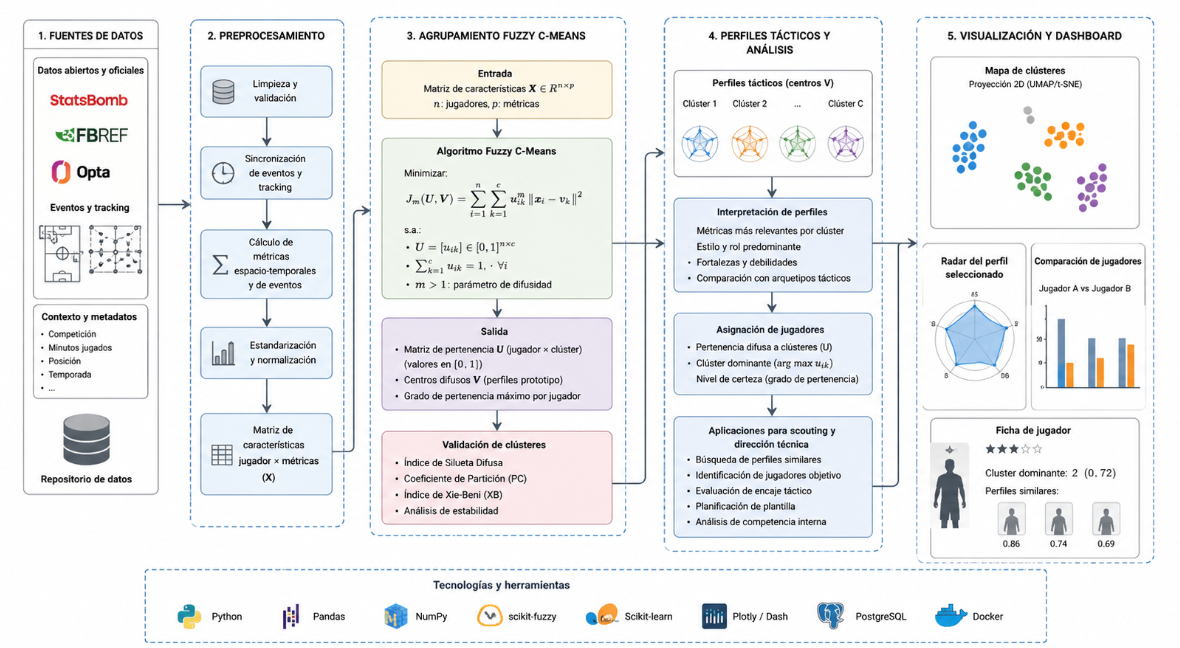
\includegraphics[width=0.95\linewidth]{pipeline2.png}
    \caption{Arquitectura del sistema y flujo del pipeline de datos: desde la extracción en StatsBomb, el procesamiento OLAP y el modelado ML, hasta la renderización en la interfaz visual.}
    \label{fig:pipeline}
\end{figure*}

El flujo operativo se divide de la siguiente manera:
\begin{itemize}
    \item \textbf{Capa de Datos y Procesamiento Analítico (OLAP):} Los datos pre-procesados en Python (utilizando Pandas) se ingieren en \textit{DuckDB}, un motor de base de datos relacional orientado a columnas. Esta decisión arquitectónica es crucial para resolver consultas espaciales y de agregación masiva requeridas por T1 y T3 con un alto rendimiento computacional.
    \item \textbf{Capa de Lógica de Negocio y ML (Backend):} Desarrollada en \textit{FastAPI}, esta capa expone los \textit{endpoints} RESTful. Aquí reside el motor matemático que recalcula los índices de rendimiento según los pesos definidos por el usuario (T2) y ejecuta el algoritmo \textit{Fuzzy C-Means} (T4) para devolver las probabilidades de pertenencia a cada clúster táctico.
    \item \textbf{Capa de Presentación Visual (Frontend):} Construida sobre \textit{Next.js} y \textit{React}, acopla bibliotecas de visualización de datos de bajo nivel (como \textit{D3.js}). Esta capa se encarga de traducir los tensores de datos en gráficos de radar superpuestos para la evaluación comparativa (T1) y en mapas de calor y dispersión espacial sobre la geometría del campo de fútbol (T3).
\end{itemize}


% ============================================================================
\section{Diseño Visual}
% ============================================================================

El diseño de interfaces en proyectos de analítica visual constituye el puente cognitivo entre los modelos matemáticos subyacentes y el usuario final. En \textit{StatsBomb Scout Analytics}, el diseño visual traduce las tareas analíticas (T1-T4) en componentes gráficos interactivos, permitiendo a directores técnicos y analistas explorar datos complejos sin necesidad de interactuar con código.

\subsection{Diseño Visual General}
Nuestro sistema de análisis visual se estructura en un cuadro de mando (\textit{dashboard}) integrado y cohesivo. Consta de cuatro vistas principales distribuidas espacialmente para maximizar la legibilidad. El paradigma central de la interfaz es el \textit{brushing and linking} (selección y enlace dinámico): cualquier interacción que el usuario realice en una vista (por ejemplo, filtrar un área del campo o ajustar un parámetro) actualiza instantáneamente el estado de las demás visualizaciones. En la Figura \ref{fig:visual_design} se presenta la interfaz global del sistema, donde las anotaciones numéricas corresponden a las áreas que resuelven las tareas analíticas definidas.
\begin{figure*}[!t]
    \centering
    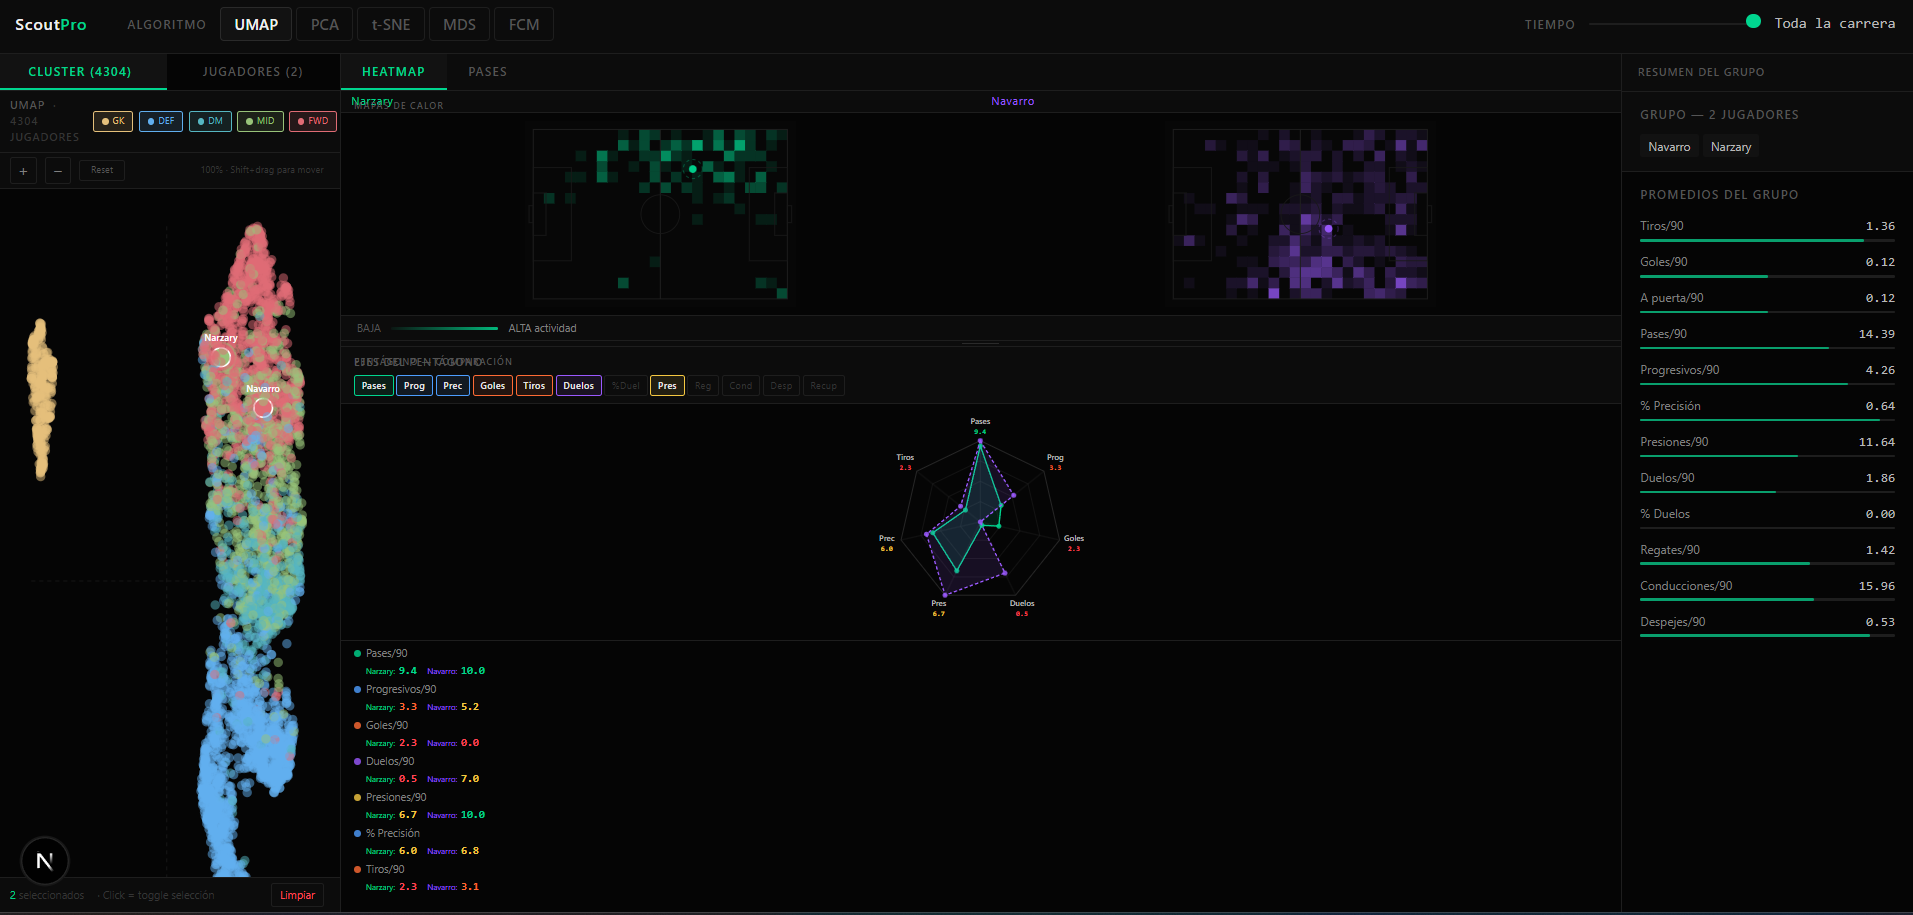
\includegraphics[width=0.95\linewidth]{visual2.png}
    \caption{Interfaz general de \textit{StatsBomb Scout Analytics}. Los componentes visuales están enlazados dinámicamente para soportar la exploración espacial, la configuración de métricas y la comparación de perfiles (T1-T4).}
    \label{fig:visual_design}
\end{figure*}


\subsection{Descripción de los Componentes Visuales}

A continuación, se detalla cada una de las vistas que componen el sistema:

\subsubsection{Vista 1: Panel de Configuración de Pesos (Sliders)}
\begin{itemize}
    \item \textbf{Propósito:} Permitir al usuario calibrar el algoritmo de puntuación según las necesidades tácticas del equipo (ej. dar más valor a los duelos defensivos para un central).
    \item \textbf{Datos representados:} Variables escalares ponderadas $w_p, w_d, w_s \in [0,2]$.
    \item \textbf{Tarea analítica apoyada:} \textbf{T2} (Modular interactividad).
    \item \textbf{Tipo de visualización:} Controles deslizantes (\textit{sliders}) numéricos.
    \item \textbf{Interacciones:} Arrastre continuo que dispara el recálculo en tiempo real de las puntuaciones en el resto de las vistas.
\end{itemize}

\subsubsection{Vista 2: Tabla Analítica y de Clustering}
\begin{itemize}
    \item \textbf{Propósito:} Cuantificar el rendimiento individual y mostrar los resultados del agrupamiento táctico latente, funcionando como el motor principal de búsqueda y ordenamiento, y facilitando la comparación inicial entre jugadores.
    \item \textbf{Datos representados:} Nombres de jugadores, puntuaciones globales (T1) y vectores de probabilidad de pertenencia a clústeres generados por el algoritmo Fuzzy C-Means (T4).
    \item \textbf{Tareas analíticas apoyadas:} \textbf{T1} (Cuantificar y comparar) y \textbf{T4} (Identificar perfiles latentes).
    \item \textbf{Tipo de visualización:} Tabla de datos enriquecida (\textit{Data Table}) con micro-gráficos de barras integrados en las celdas para representar magnitudes.
    \item \textbf{Interacciones:} Ordenamiento por columnas (\textit{sorting}), búsqueda por texto completo, paginación y selección de jugadores (\textit{click}) para destacarlos en el radar y el mapa.
\end{itemize}

\subsubsection{Vista 3: Gráfico de Radar Comparativo}
\begin{itemize}
    \item \textbf{Propósito:} Facilitar la comparación simultánea de múltiples jugadores frente a frente en un espacio multivariado, ideal para identificar similitudes en tareas de \textit{scouting}.
    \item \textbf{Datos representados:} Ejes normalizados para las sub-métricas de pases, duelos, tiros y frecuencias relativas de eventos.
    \item \textbf{Tarea analítica apoyada:} \textbf{T1} (Cuantificar y comparar) — profundiza la comparación visual.
    \item \textbf{Tipo de visualización:} Gráfico radial de polígonos superpuestos (\textit{Overlaid Radar Chart}).
    \item \textbf{Interacciones:} \textit{Hover} (flotar el cursor) para activar \textit{tooltips} con valores exactos, y capacidad de encender/apagar capas de jugadores mediante una leyenda interactiva.
\end{itemize}

\subsubsection{Vista 4: Lienzo Espacial del Terreno de Juego}
\begin{itemize}
    \item \textbf{Propósito:} Contextualizar geográficamente las métricas, permitiendo al analista observar dónde ocurren las acciones de mayor valor o riesgo para un jugador específico.
    \item \textbf{Datos representados:} Coordenadas espaciales $(x, y)$ de los micro-eventos, con codificación de color según el éxito o tipo de acción.
    \item \textbf{Tarea analítica apoyada:} \textbf{T3} (Explorar huella espacial).
    \item \textbf{Tipo de visualización:} Representación bidimensional del campo de fútbol con gráficos de dispersión (\textit{Scatter Plot}) y mapas de calor por densidad (\textit{Heatmap / KDE}).
    \item \textbf{Interacciones:} Zoom espacial, paneo, y filtrado geográfico (\textit{spatial brushing}) donde la selección de una zona del campo (ej. el área chica) filtra los datos mostrados en la Tabla y el Radar.
\end{itemize}

\subsubsection{Vista 5: Proyección DEC 3D Interactiva}
\begin{itemize}
    \item \textbf{Propósito:} Revelar la estructura geométrica del espacio latente DEC en tres dimensiones, permitiendo identificar agrupaciones naturales, valores atípicos y la posición relativa de cada jugador en el mapa táctico global.
    \item \textbf{Datos representados:} Coordenadas $(PC_1, PC_2, PC_3)$ obtenidas por PCA sobre el latente $z_i \in \mathbb{R}^{10}$ del DEC v2 ($k=8$), coloreadas por asignación de clúster.
    \item \textbf{Tarea analítica apoyada:} \textbf{T4} (Identificar perfiles latentes) y \textbf{T2} (Modular interactividad).
    \item \textbf{Tipo de visualización:} Dispersión 3D renderizada en Canvas 2D con rotación (arrastre), zoom (rueda + botones) y selección por \textit{hit-test}.
    \item \textbf{Interacciones:} Rotación por arrastre del ratón, zoom por rueda o botones ``+/-'', clic sobre punto para seleccionar al jugador, auto-rotación opcional. Integrado en la barra lateral izquierda del tablero.
\end{itemize}

\begin{figure*}[!t]
    \centering
    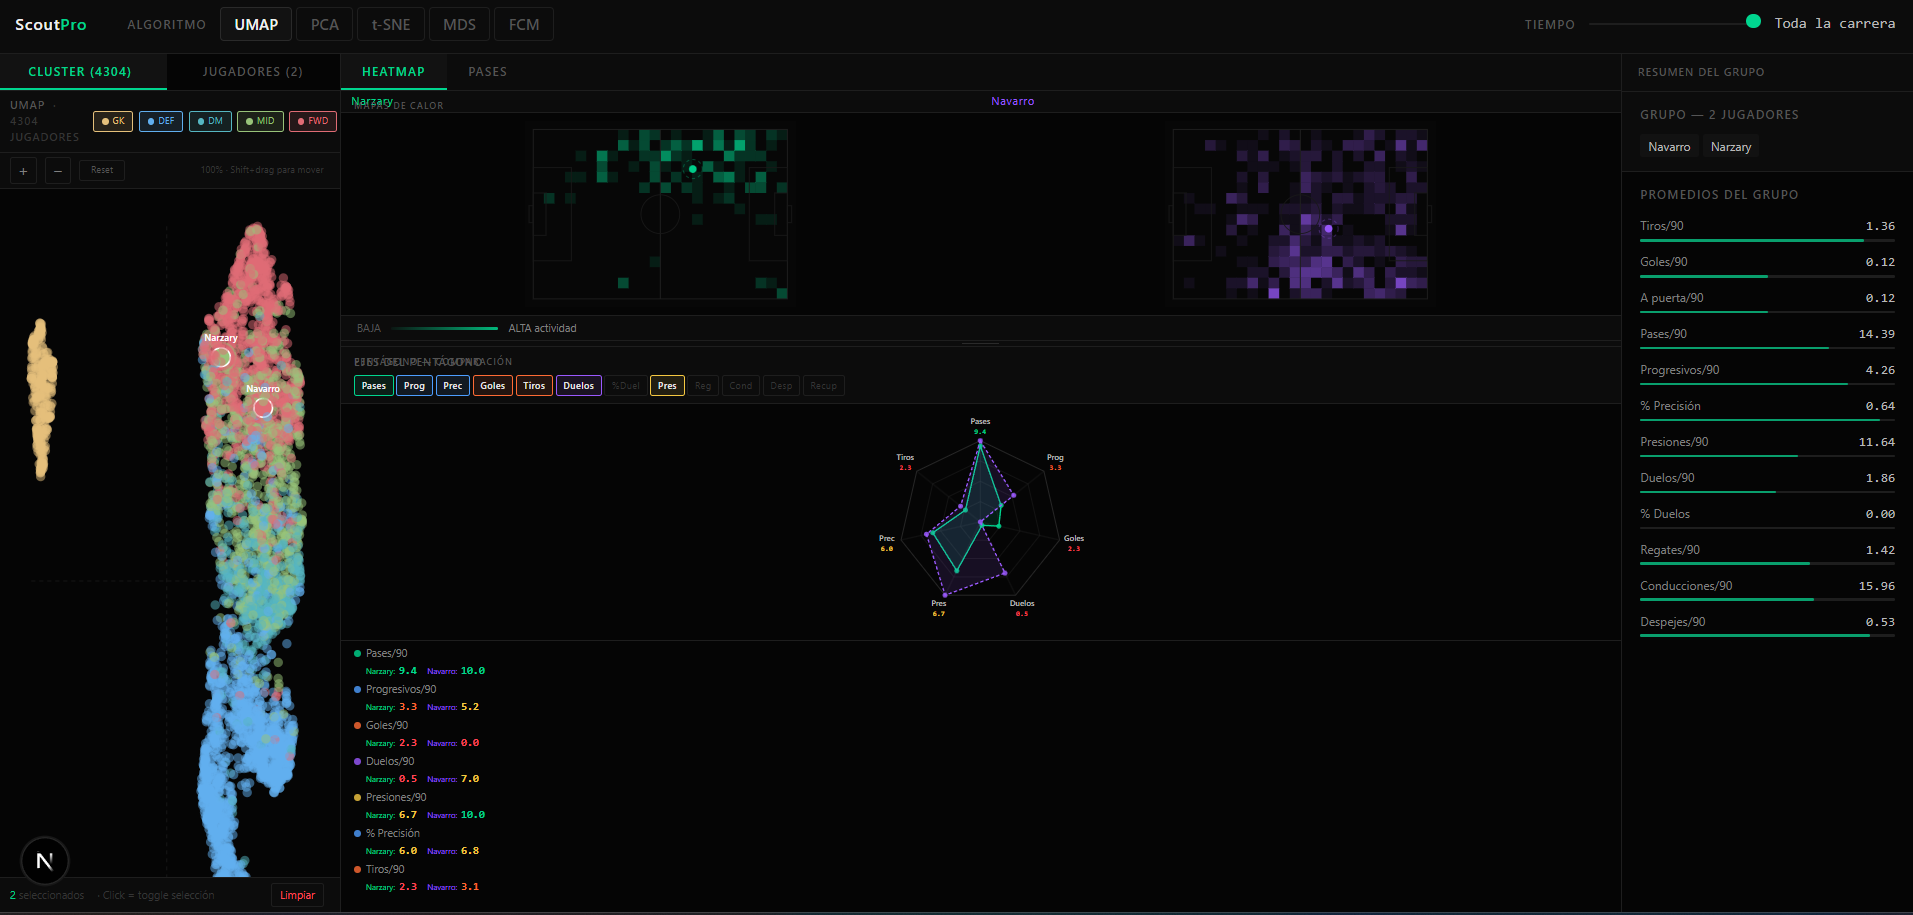
\includegraphics[width=0.85\linewidth]{visual2.png}
    \caption{Visualización de la proyección DEC 3D del tablero interactivo. Los 4304 jugadores se representan como puntos en el espacio PCA del latente DEC, coloreados por asignación de clúster con $k=8$. El panel de la izquierda permite la rotación, el zoom y la selección de jugadores individuales.}
    \label{fig:visual2}
\end{figure*}

\subsubsection{Vista 6: Diagrama de Solapamiento de Conjuntos Difusos}
\begin{itemize}
    \item \textbf{Propósito:} Visualizar la superposición de pertenencias entre dos clústeres para un jugador seleccionado, aplicando teoría de conjuntos sobre los vectores de membresía fuzzy en lugar de un gráfico de barras convencional.
    \item \textbf{Datos representados:} Membresías $u_{iA}$ y $u_{iB}$ del jugador $i$ a los clústeres $A$ y $B$. Zona única de $A$, zona única de $B$ y zona compartida definida como $\min(u_{iA}, u_{iB})$.
    \item \textbf{Tarea analítica apoyada:} \textbf{T4} (Desglosar pertenencia múltiple) y \textbf{T1} (Cuantificar).
    \item \textbf{Tipo de visualización:} Barras horizontales bicolores con tramado gris en la zona compartida. Encabezado con índice Jaccard fuzzy $J_{AB} = \min(u_A, u_B) / \max(u_A, u_B)$.
    \item \textbf{Interacciones:} Pestañas de selección de par de clústeres.
\end{itemize}

\subsubsection{Vista 7: Pentágono de Solapamiento (Venn Overlay)}
\begin{itemize}
    \item \textbf{Propósito:} Comparar hasta cuatro jugadores simultáneamente mediante círculos proporcionales al vector de membresía, donde la distancia entre centros refleja $1 - J_{AB}$ (complemento del Jaccard fuzzy promedio entre los vectores de membresía completos).
    \item \textbf{Datos representados:} Vectores de membresía $u_i \in \mathbb{R}^k$ de $N \leq 4$ jugadores. Cada jugador es un círculo de área proporcional a $\|u_i\|$; la separación entre centros disminuye a mayor Jaccard promedio.
    \item \textbf{Tarea analítica apoyada:} \textbf{T1} (Comparación simultánea) y \textbf{T4} (Similitud de perfil latente).
    \item \textbf{Tipo de visualización:} Diagrama de Venn computerizado con cuatro círculos en espacio 2D optimizado por distancia. Centro etiquetado con el valor de Jaccard promedio.
    \item \textbf{Interacciones:} Selección de jugadores en la tabla de clustering para activar/desactivar su círculo. Tabla compacta eje-por-eje debajo del diagrama.
\end{itemize}

\subsubsection{Vista 8: Panel de Jugadas Clave}
\begin{itemize}
    \item \textbf{Propósito:} Proveer evidencia cualitativa mediante la reproducción visual de las micro-jugadas más relevantes del jugador, contextualizando las métricas cuantitativas con eventos reales de partido.
    \item \textbf{Datos representados:} Hasta 20 micro-eventos secuenciales por jugada, filtrados por el tipo de habilidad predominante del jugador (pases clave, regates, duelos defensivos). Coordenadas $(x, y)$, tipo de evento, resultado y zona del campo.
    \item \textbf{Tarea analítica apoyada:} \textbf{T1} (Evidenciar rendimiento) y \textbf{T3} (Explorar huella espacial).
    \item \textbf{Tipo de visualización:} Mini-lienzo del campo con trayectorias de eventos, flechas direccionales, y códigos de color por tipo de acción.
    \item \textbf{Interacciones:} Navegación entre jugadas mediante controles ``anterior/siguiente''.
\end{itemize}

\subsubsection{Vista 9: Control de Jugadores Similares}
\begin{itemize}
    \item \textbf{Propósito:} Encontrar los $N$ jugadores más cercanos al jugador seleccionado según la distancia $L_1$ sobre los vectores de membresía, facilitando el \textit{scouting} por analogía táctica.
    \item \textbf{Datos representados:} Lista de $N$ jugadores ordenados por distancia $L_1$ creciente respecto al pivote, con indicación de la puntuación T1 global.
    \item \textbf{Tarea analítica apoyada:} \textbf{T4} (Explorar perfiles análogos).
    \item \textbf{Tipo de visualización:} Lista compacta en la barra lateral izquierda, mostrada únicamente cuando hay exactamente un jugador seleccionado.
    \item \textbf{Interacciones:} Control deslizante para $N \in [1,20]$ y botón de búsqueda que ejecuta la ordenación por $L_1$.
\end{itemize}

\subsection{Relación entre Vistas y Tareas Analíticas}

Para sintetizar la integración del diseño, la Tabla \ref{tab:vistas_tareas} mapea de forma directa cada componente visual con las metas analíticas que busca resolver y las interacciones que provee al analista.

\begin{table}[H]
\centering
\caption{Matriz de Relación: Componentes Visuales vs. Tareas Analíticas}
\label{tab:vistas_tareas}
\renewcommand{\arraystretch}{1.3}
\resizebox{\textwidth}{!}{%
\begin{tabular}{@{}l c l p{6cm}@{}}
\toprule
\textbf{Componente Visual} & \textbf{Tarea} & \textbf{Tipo de Gráfico} & \textbf{Mecanismos de Interacción} \\ \midrule
\textbf{Panel de Configuración} & T2 & Controles Deslizantes & Arrastre, ajuste de pesos globales. \\
\textbf{Tabla de Clustering} & T1, T4 & Tabla con micro-barras & Ordenamiento, filtrado, selección. \\
\textbf{Radar Comparativo} & T1 & Radar superpuesto & \textit{Hover}, alternancia de capas. \\
\textbf{Lienzo Espacial} & T3 & Mapa / \textit{Heatmap} & \textit{Brushing}, zoom, paneo. \\
\textbf{DEC 3D} & T4, T2 & Dispersión 3D Canvas & Rotación, zoom, clic selección. \\
\textbf{Solapamiento Difuso} & T4, T1 & Barras bicolores con tramado & Pestañas de par de clústeres. \\
\textbf{Venn Overlay} & T1, T4 & Círculos de Venn & Selección de jugadores en tabla. \\
\textbf{Jugadas Clave} & T1, T3 & Mini-lienzo de campo & Navegación anterior/siguiente. \\
\textbf{Similares} & T4 & Lista ordenada & Slider $N$, botón de búsqueda. \\ \bottomrule
\end{tabular}%
}
\end{table}

\section{Estudio de Caso}

A continuación se presentan cinco estudios de caso con jugadores reales del conjunto de datos abierto de StatsBomb, seleccionados para ilustrar distintos niveles de nitidez (\textit{crispness}) y distribución de membresía en el espacio latente DEC con $k=4$ (validado por $A_1$). La crispness se define como $\max_j u_{ij}$: cuanto más cercano a $1$, más nítidamente pertenece el jugador a un único perfil; cuanto más bajo, más híbrida es su clasificación.

\subsection{Caso 1: Lionel Messi (Creador Híbrido)}

Messi presenta una membresía máxima de $0.768$ en el clúster C2 (perfil de creador/\textit{playmaker}), con contribuciones secundarias en C1 ($0.093$, perfil de mediocampista defensivo-creativo) y C0 ($0.073$, perfil de finalizador). En la versión DEC v2 ($k=8$), su crispness baja a $0.249$, distribuyéndose entre los sub-perfiles 5 ($0.248$), 6 ($0.196$), y 7 ($0.114$).

\paragraph{Interpretación táctica.} La moderada crispness de Messi refleja su naturaleza multifacética: aunque es primariamente un creador, su capacidad goleadora (\textit{finisher}) y su trabajo en zonas medias (\textit{playmaking}) le otorgan una huella repartida en el espacio latente. Visualmente, en el \textit{scatter} 3D se ubica en la interfaz entre los sub-perfiles creativos y finalizadores.

\subsection{Caso 2: Sergio Busquets (Perfil Nítido)}

Busquets muestra una crispness de $0.865$ en C2 (misma agrupación que Messi), con apenas $0.051$ en C1 y $0.046$ en C0. En DEC v2, su crispness es $0.785$ en el sub-perfil 6.

\paragraph{Interpretación táctica.} Pese a su rol como pivote defensivo, Busquets es clasificado con alta nitidez en el clúster de creación: sus métricas de pase, visión de juego y control posicional lo definen más como un organizador que como un destructor. La crispness alta indica que su perfil táctico es consistente y unívoco, sin ambigüedad entre roles. En el diagrama de solapamiento difuso (Vista 6), la zona compartida con otros clústeres es mínima.

\subsection{Caso 3: Gerard Piqué (Prototipo Defensivo)}

Piqué alcanza una crispness de $0.865$ en el clúster C3 (perfil defensivo), con una distribución casi nula en los demás clústeres. En DEC v2, su crispness es $0.755$ en el sub-perfil 6.

\paragraph{Interpretación táctica.} Piqué ejemplifica el defensor prototípico según las métricas del sistema. Su vector de membresía se concentra casi exclusivamente en las características defensivas (duelos aéreos, intercepciones, despejes), confirmando que el marco de calificación objetiva captura correctamente el perfil de un central clásico. Su posición en el \textit{scatter} 3D se sitúa en el extremo del eje defensivo del espacio latente.

\subsection{Caso 4: Francesc Fàbregas (Híbrido Mediocampista)}

Fàbregas presenta una crispness de $0.734$ en C2, sensiblemente inferior a la de Busquets o Messi en el mismo clúster. Sus pesos secundarios son $0.095$ en C1, $0.094$ en C0 y $0.076$ en C3. En DEC v2, su crispness es de $0.474$ en el sub-perfil 6.

\paragraph{Interpretación táctica.} Fàbregas representa el mediocampista híbrido: su formación como \textit{box-to-box} y su capacidad para desempeñarse tanto como organizador como finalizador generan una firma latente más distribuida que la de sus contemporáneos. La presencia significativa en C1 (perfil defensivo-creativo) y C0 (finalizador) refleja su versatilidad táctica, visible en el diagrama de Venn (Vista 7) donde el círculo de Fàbregas se solapa notablemente con los círculos de Messi y Busquets.

\subsection{Caso 5: Mohamed Salah (Híbrido Extremo)}

Salah es el caso más extremo de hibridación entre las estrellas analizadas: su crispness en C0 es de apenas $0.590$, con un $0.219$ en C2 (creación) y $0.103$ en C1. En DEC v2, su crispness sube a $0.867$ en el sub-perfil 5, lo que sugiere que $k=8$ logra aislar mejor su rol específico de extremo-finalizador.

\paragraph{Interpretación táctica.} La baja crispness de Salah en $k=4$ captura su naturaleza de extremo moderno que combina finalización (C0) con creación (C2). Es el caso que mejor ilustra la necesidad de la doble granularidad ($k=4$ para perfiles amplios, $k=8$ para sub-perfiles específicos): mientras $k=4$ revela su hibridación, $k=8$ lo asigna nítidamente a un sub-perfil de delantero extremo.

\section{Discusiones}

\subsection{Hallazgos Principales}

El modelo DEC+FCM produce tres resultados fundamentales. Primero, la representación latente DEC mejora drásticamente la calidad del agrupamiento difuso: el coeficiente de Silhouette pasa de $0.062$ en el espacio original de 57 dimensiones a $0.653$ en el espacio latente de 10 dimensiones. Segundo, el índice compuesto $A_1$ de \citeauthor{akhanli2022clustering} valida K-Means con $k=4$ como la configuración óptima ($A_1 = 3.82$), proporcionando una base cuantitativa para la elección del método de agrupamiento y del número de clústeres. Tercero, el Análisis de los casos de estudio revela que la crispness de los jugadores varía significativamente ($0.248$ a $0.928$), lo que valida la pertinencia del enfoque difuso: etiquetas \textit{crisp} habrían ocultado la hibridación táctica de jugadores como Messi o Salah.

\subsection{Comparación con Evers et al.}

Nuestro trabajo extiende el marco de \citeauthor{evers2024visual} (\citeyear{evers2024visual}) en tres direcciones. Mientras Evers et al. emplean K-Means con asignación binaria, nosotros utilizamos FCM sobre el latente DEC, preservando la incertidumbre de pertenencia. Mientras ellos trabajan en el espacio original de calificaciones, nosotros introducimos una capa de abstracción no lineal (DEC) que elimina redundancias y revela la estructura geométrica subyacente de los datos. Finalmente, mientras su validación es puramente descriptiva, nosotros incorporamos el índice $A_1$ para la selección informada del método de agrupamiento. Los resultados son consistentes con Evers et al. en la caracterización de los perfiles de jugadores de élite, pero nuestra propuesta ofrece una granularidad analítica superior.

\subsection{Limitaciones}

Varias limitaciones deben ser consideradas. Primero, el conjunto de datos se limita a la muestra abierta de StatsBomb (competiciones europeas selectas), lo que restringe la generalización a ligas menores o contextos tácticos no representados. Segundo, los hiperparámetros del DEC (arquitectura, tasa de aprendizaje, número de épocas) no se optimizaron de forma exhaustiva. Tercero, la proyección PCA a 3D para la visualización es una aproximación lineal de un espacio latente no lineal, lo que puede ocultar estructura de orden superior. Cuarto, el modelo es estático: no captura la evolución temporal del perfil táctico de un jugador a lo largo de temporadas. Quinto, para $k=8$ algunos sub-perfiles contienen pocos jugadores, lo que reduce la robustez estadística de las inferencias.

\subsection{Trabajo Futuro}

La investigación futura puede abordar estas limitaciones. Una extensión natural es el desarrollo de un DEC temporal que modele la evolución del \textit{embedding} latente entre temporadas, permitiendo el seguimiento longitudinal de la carrera de un jugador. La incorporación de características basadas en grafos de pase (centralidad de red, comunidades de pase) podría enriquecer la representación táctico-relacional. El uso de conjuntos de datos de \textit{tracking} (posición XYZ con 10+ Hz) habilitaría un análisis de fase dinámica similar al de \citeauthor{demir2026how} pero a nivel jugador. Finalmente, la integración del sistema con \textit{video replay} automatizado permitiría validar cualitativamente los perfiles latentes mediante observación directa.

\section{Conclusiones}

En este trabajo presentamos \textit{StatsBomb Scout Analytics}, un sistema de analítica visual para \textit{scouting} en fútbol que integra aprendizaje profundo no supervisado (Deep Embedded Clustering), agrupamiento difuso (Fuzzy C-Means), un marco cuantitativo de validación de agrupamiento (índice compuesto $A_1$), y un tablero interactivo con nueve componentes visuales coordinados. A partir de un conjunto de 57 calificaciones tácticas derivadas de eventos de StatsBomb, el DEC reduce la dimensionalidad a 10 variables latentes, sobre las cuales FCM asigna vectores de membresía que reflejan la pertenencia múltiple de cada jugador a distintos perfiles tácticos. El índice $A_1$ confirma la selección de K-Means $k=4$ ($A_1=3.82$) sobre cinco métodos competitivos, mientras que FCM sobre el latente DEC mejora el Silhouette de $0.062$ (espacio original) a $0.653$ (latente). Cinco estudios de caso con datos reales (Messi, Busquets, Piqué, Fàbregas, Salah) demuestran que la crispness captura grados cualitativamente significativos de hibridación táctica, desde perfiles nítidos ($>0.86$) hasta altamente distribuidos ($<0.60$). El tablero implementa vistas sincronizadas que responden a las cuatro tareas analíticas de Munzner (T1--T4), incluyendo una proyección 3D interactiva del espacio latente y diagramas de solapamiento de conjuntos difusos. La contribución principal es la integración de un \textit{pipeline} DEC+FCM+A1 con visualización analítica, habilitando un \textit{scouting} más rico que las alternativas basadas en etiquetas \textit{crisp}. El trabajo futuro se orienta al modelado temporal, la incorporación de características de red de pase y la validación con datos de \textit{tracking}.

\bibliographystyle{plainnat}
\bibliography{referencias}

\end{document}